\section{Development}

Each component of the project had to be developed individually before assembling them together into a working prototype. The Raspberry Pi, the router, the Sensor Tag and the TelosB. A description of each devices configuration will be described and then how the connection is made between each of them.\\

A good overview of the project can be seen in Figure \ref{fig:over}.

\begin{figure}[!h]
	\begin{center}
		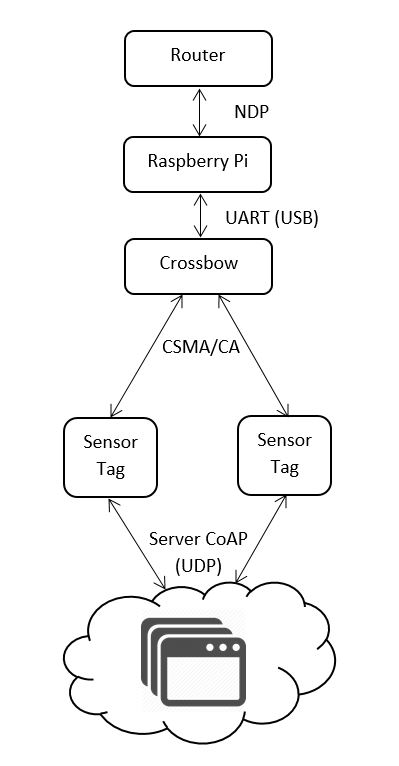
\includegraphics[width=0.6\linewidth]{protocol}
		\caption{sensor node connected with the debugger to a computer}
		\label{fig:over}
	\end{center}
\end{figure} 

\subsection{Raspberry pi - 6LoWPAN Boarder Router}

The Raspberry Pi acts as a boarder router for the WSN in Smart brigde mode. It mitigates information to from the WSN mesh into the IPv6 network of the router. The boarder router is installed into the Raspberry pi via the 6LBR-1.3.3 Packages for Raspian. The service can be started through the terminal and the status of the working service can be seen in Figure \ref{fig:router}.

\begin{lstlisting}[basicstyle=\small,language=bash,caption={Start the 6lbr service and check the status}]

$ sudo 6lbr service start
$ sudo service 6lbr status
  6lbr.service - LSB: 6LoWPAN Border Router
Loaded: loaded (/etc/init.d/6lbr)
Active: active (running); 1h 32min ago
\end{lstlisting}

After making sure that the bridge boarder router is configured correctly (see the documentation on the 6lbr github page for configuring a rapsberry pi connection), the TelosB should be connected the the Raspberry Pi and the IPv6 address can be found be running: 
 
\begin{lstlisting}[basicstyle=\small,language=bash,caption={Get the TelosB node IPv6 address for accessing the 6lbr client}]

$ cat /var/log/6lbr.ip 
2002:aaa:2e10:10:212:7400:13ea:961
\end{lstlisting}

This address can then be used to access the 6lbr client directly as seen in Figure \ref{fig:interface}.

\begin{figure}[!h]
	\begin{center}
		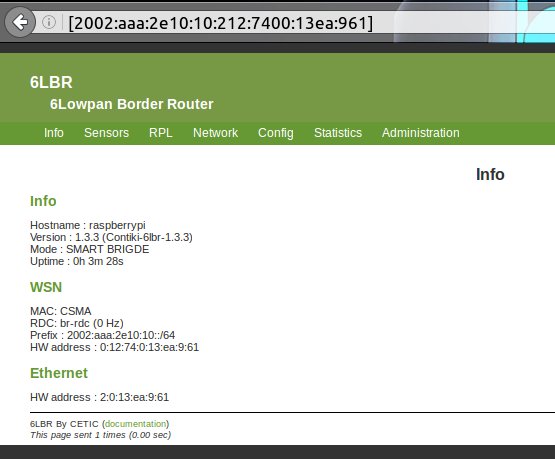
\includegraphics[width=1\linewidth]{interface}
		\caption{The 6lbr interface on the pi}
		\label{fig:interface}
	\end{center}
\end{figure} 

\subsection{Router}

The router has to be configured to IPv6 network as well to be able to communicate with the 6LoWPAN network and assign IPv6 addresses to devices that want to access the nodes via CoAP, even mobile phones. The router was configured to 6to4 (converting IPv6 to IPv4 traffic), see Figure \ref{fig:routerSettings} with RADVD.

\begin{figure}[!h]
	\centering
		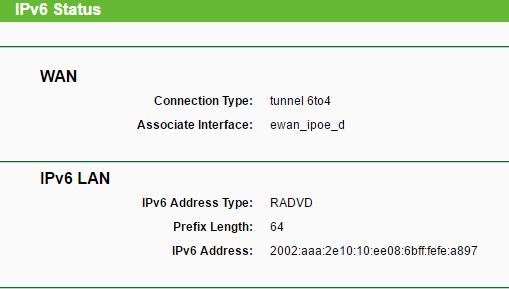
\includegraphics[width=1\linewidth]{routerSettings}
		\caption{The router settings needed for communicating within the LAN to the WSN}
		\label{fig:routerSettings}
\end{figure} 

\subsection{TI Sensor Tag - Sensor nodes}

The sensor tag communicates to the TelosB via 802.15.4. For working with the tag, a special software (Windows only) has to be used to upload a binary file to it see the next Section \ref{sec:flash}. First the code that is supposed to be used has to be cross compiled on a Linux machine. For the communication with the TelosB, the contiki library was used for the sensor tags processor family, more specific: "/contiki/examples/cc26xx/cc26xx-web-demo/cc26xx-web-demo.c". In order to compile it the following command should be run:

\begin{lstlisting}[basicstyle=\small,language=bash,caption={Cross compiling the web-demo to a binary file for the sensor tag}]

cd contiki/examples/cc26xx/cc26xx-web-demo/
nano project-conf.h
make TARGET=srf06-cc26xx BOARD=sensortag/cc2650
     cc26xx-web-demo.bin CPU_FAMILY=cc26xx
\end{lstlisting}

\begin{lstlisting}[basicstyle=\small,language=c,caption={The configurisation file for the web-demo in directory: contiki/examples/cc26xx/cc26xx-web-demo/project-confg.h}]

#define RF_BLE_CONF_ENABLED                 0
#define CC26XX_WEB_DEMO_CONF_MQTT_CLIENT    0
#define CC26XX_WEB_DEMO_CONF_6LBR_CLIENT    0
#define CC26XX_WEB_DEMO_CONF_COAP_SERVER    1
#define CC26XX_WEB_DEMO_CONF_NET_UART       0
\end{lstlisting}

These commands create a binary file "cc26xx-web-demo.bin" which can be flashed onto the sensor tag via the SmartRF Flash Programmer 2.


\subsubsection{Flashing the Texas Instrument Sensor-Tag} 
\label{sec:flash}
In order to flash the sensor tag, SmartRF Flash Programmer 2 made by Texas Instrument has been used. For flashing the node a sensor tag needs a Debugger DevPack, the debugger allows for communication to the sensor via USB as it is shown in Figure \ref{fig:debug}.  
\begin{figure}[!h]
	\begin{center} 	
		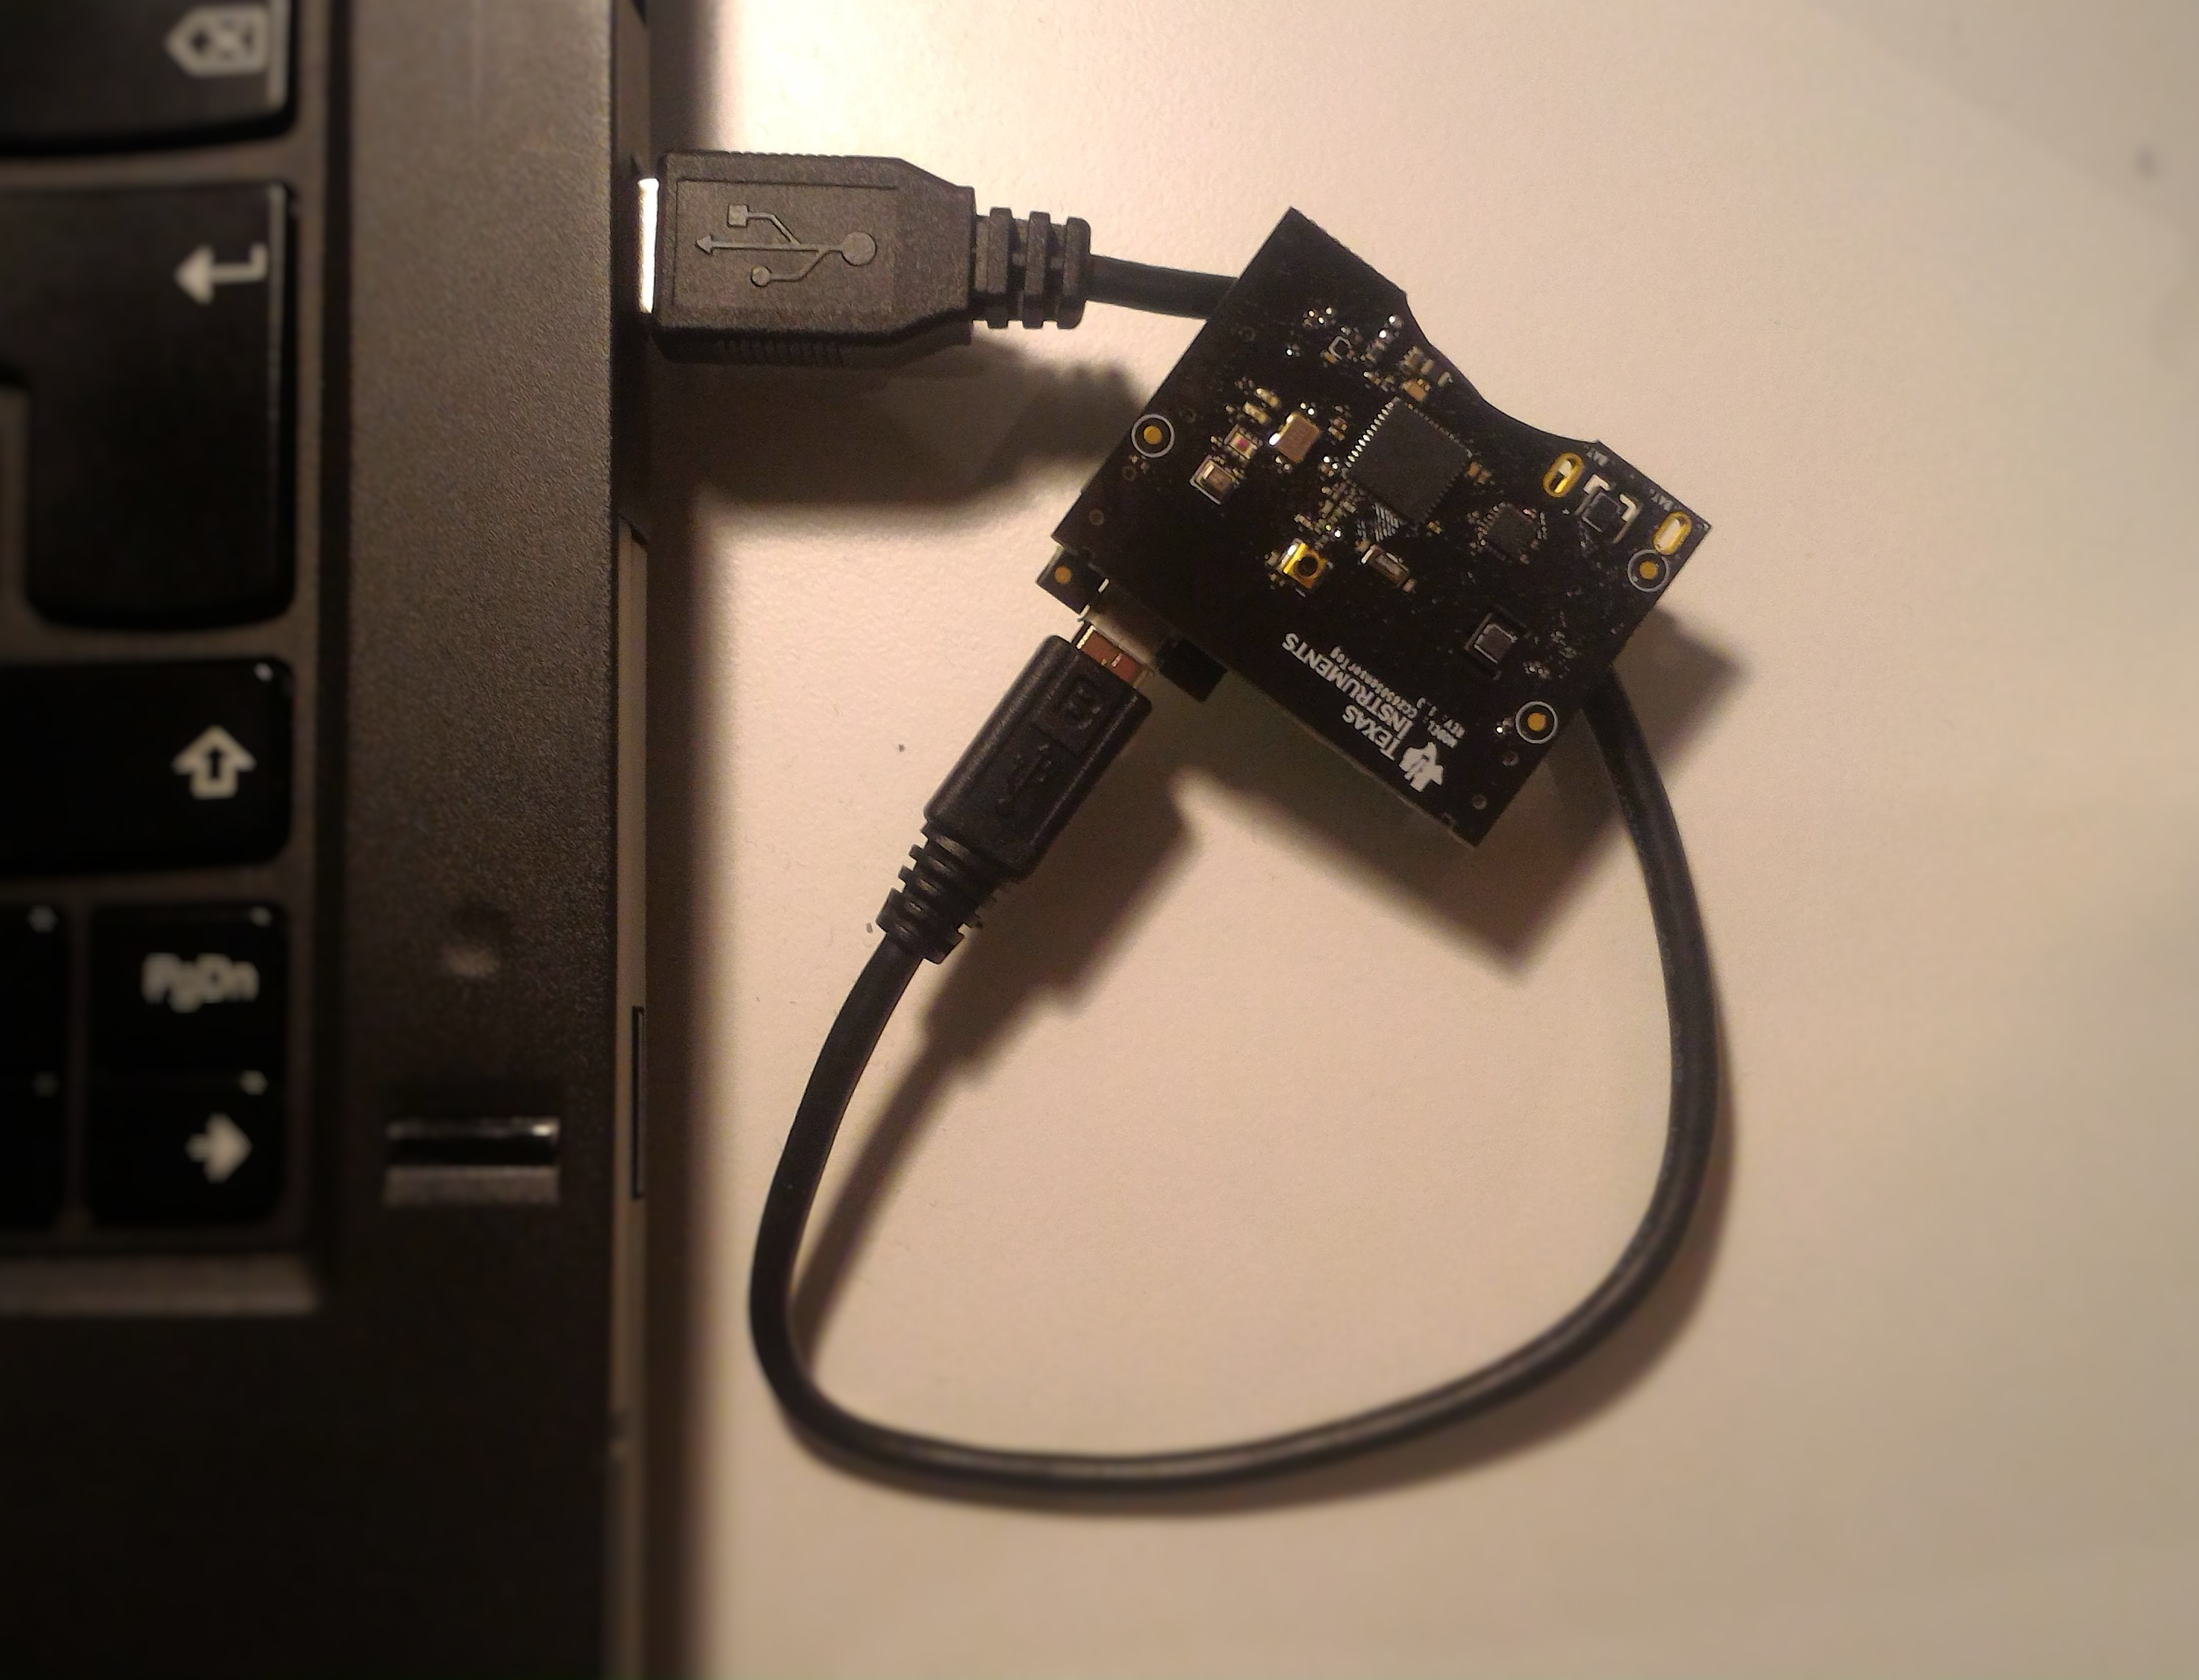
\includegraphics[width=0.8\linewidth]{debugger}
		\caption{sensor node connected with the debugger to a computer}
		\label{fig:debug}
	\end{center}
\end{figure} 

\subsection{Crossbow TelosB mote - slip-radio}
This allows the Pi to act as a network coordinator for the sensor tags in the 6loWPAN network via the 802.15.4 enabled transceiver on the Crossbow. The software on the Crossbow is a slip-radio, specially made for it by Contiki. This